\documentclass[10pt,conference]{IEEEtran}

\usepackage{graphicx}
\usepackage{tikz}
\usepackage{amsmath}
\usepackage{cite}

\title{Selective Prior-Conditioned State-Space Model (SPC-SSM) for Remote Sensing Change Detection}

\author{
    \IEEEauthorblockN{
        Yosra Naceur\IEEEauthorrefmark{1}, 
        Mariem Zaouali\IEEEauthorrefmark{2}, 
        Sonia Bouzidi\IEEEauthorrefmark{3}
    }
    \IEEEauthorblockA{
        \IEEEauthorrefmark{1}Affiliation of Yosra Naceur\\
        \IEEEauthorrefmark{2}Affiliation of Mariem Zaouali\\
        \IEEEauthorrefmark{3}Affiliation of Sonia Bouzidi
    }
}

\begin{document}
\maketitle

\begin{abstract}
 To monitor Earth's surface modifications, high-resolution imagery provides rich textural and geometric details used to analyze changes between bi-temporal images acquired at different times. However, inherent spectral heterogeneity complicates the distinction between relevant changes and noise. To address the limitations of traditional algebraic and transformation-based methods, Deep Learning architectures have been widely adopted for automated semantic feature extraction. Despite these advancements, existing models—particularly those based on the conventional U-Net structure—often struggle with edge integrity and the internal holes phenomenon within change features. To enhance performance, guided change detection and attention mechanisms have been introduced to help networks focus on salient information. Unfortunately, these mechanisms inherently suffer from severe computational complexity. To address these limitations, we propose the Prior-Conditioned State-Space Model (SPC-SSM), an architecture that fundamentally refactors multiscale feature fusion. Instead of relying on simple feature concatenation or computationally heavy self-attention, SPC-SSM utilizes deep semantic features to generate change maps that act as explicit prior guidance. These priors are integrated directly into a State-Space Model (Mamba) framework to condition the sequence modeling process. By steering the state transitions across different hierarchical levels, our SSM dynamically fuses multi-scale features—aggregating broad, high-level semantics with fine, low-level spatial details under linear computational complexity. This efficient, prior-guided continuous fusion overcomes the receptive field constraints of traditional networks and captures robust long-distance pixel dependencies. Extensive experiments and ablation studies on four major CD datasets demonstrate that SPC-SSM significantly improves feature expression, delivering superior precision and efficiency in detecting complex change patterns.
\end{abstract}

\begin{IEEEkeywords}
Change detection, Context Guided Module, Prior-Conditioned State-Space Model
\end{IEEEkeywords}





\section{Introduction}
Change detection (CD) from satellite imagery aims to identify surface alterations over time, serving as a foundation for land-use analysis, disaster monitoring, and sustainable urban planning. Traditional methods, including image differencing and principal component analysis, have been progressively replaced by deep learning-based techniques capable of learning complex spatial-spectral representations.

Among these, convolutional encoder-decoder networks such as U-Net \cite{ronneberger2015u} have become dominant due to their ability to capture both low-level spatial details and high-level semantics. However, these architectures often suffer from limited receptive fields and high computational cost when scaled to high-resolution imagery.
Deep convolutional neural networks (CNNs) have significantly advanced remote sensing change detection due to their strong local feature extraction capability. Early deep models adopted Siamese architectures to extract features from bi-temporal images and measure their differences. Encoder–decoder frameworks further improved performance by enabling multi-scale feature aggregation.

However, CNN-based approaches inherently rely on local receptive fields and struggle to capture long-range spatial dependencies, especially in high-resolution remote sensing imagery where contextual reasoning is essential. Although deeper networks enlarge the receptive field, they often fail to model global interactions efficiently.

To address the limitations of CNNs in modeling global context, transformer-based architectures were introduced into remote sensing change detection. Vision transformers and hybrid CNN–Transformer models have demonstrated improved capability in capturing long-range spatial dependencies.

Notably, transformer-based change detection models leverage self-attention to construct dense interaction maps between spatial positions, enabling global reasoning across the image. While effective, self-attention incurs quadratic computational complexity with respect to spatial resolution, making it computationally expensive for large-scale remote sensing imagery.


Recently, state-space models (SSMs) have emerged as an efficient alternative to attention mechanisms. The Mamba architecture \cite{gu2023mamba} reformulates sequence modeling through selective state-space propagation, achieving linear complexity while maintaining long-range modeling capacity.

Vision-oriented adaptations such as Vision Mamba \cite{zhu2024vision} extended this framework to image tasks including classification and segmentation by applying spatial selective scanning.

In the context of remote sensing change detection, several Mamba-based approaches have been proposed. For example, ChangeMamba \cite{chen2024changemamba} introduced a spatiotemporal state-space model to replace transformer-based interaction modules, demonstrating improved efficiency and competitive accuracy. Similarly, CWmamba explored a hybrid CNN–Mamba architecture, leveraging CNNs for local feature extraction and Mamba blocks for global dependency modeling.

While these methods successfully improve global perception and computational efficiency, they primarily integrate Mamba within the backbone encoder. Consequently, they focus on feature extraction rather than explicitly reformulating change-guided refinement mechanisms.


Change-guided models introduce prior change maps to guide feature refinement and suppress irrelevant background regions. Attention-based change-guided modules dynamically reweight spatial features according to estimated change probabilities.

However, such mechanisms still rely on dense attention operators or gating strategies that do not explicitly model spatial evolution dynamics. Moreover, they typically treat prior maps as static weighting masks rather than as control signals driving a structured propagation process.


In contrast to existing Mamba-based change detection methods that replace or enhance backbone feature extraction, we reinterpret change-guided attention as a structured spatial dynamical system.

We propose a Prior-Conditioned Recurrent State-Space Refinement (SPC-SSM) module that models spatial feature propagation through a stable state-space operator conditioned on a learned prior change map. Instead of constructing dense attention matrices, the proposed method dynamically propagates change information across spatial locations with linear computational complexity.

This formulation bridges change-guided attention and structured state-space modeling, yielding a principled and computationally efficient refinement mechanism that operates generically in feature space and remains encoder-agnostic. While implemented within a hierarchical multi-scale framework, the proposed refinement does not depend on the internal design of the backbone and can be seamlessly integrated into CNN-, Transformer-, or SSM-based encoders that provide intermediate feature representations.

\section{Proposed Method}

\begin{figure*}[t]
\centering
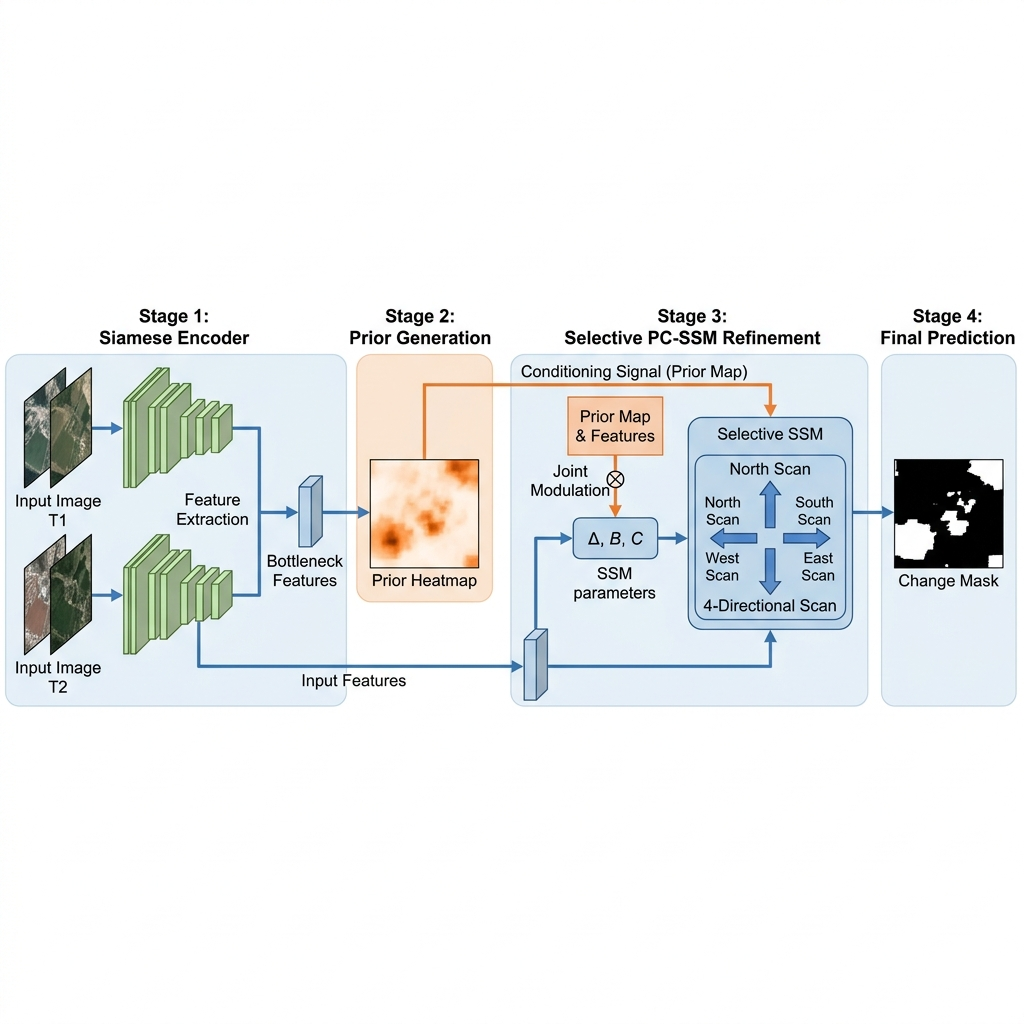
\includegraphics[width=\textwidth]{figures/pcssm_architecture.png}
\caption{Overview of the proposed Selective Prior-Conditioned State-Space Model (SPC-SSM) architecture. The model employs a Siamese encoder to extract multi-scale features. A semantic change prior is generated from the bottleneck and progressively upsampled to condition a cascade of SPC-SSM blocks, where state-space transitions are dynamically gated by the prior map.}
\label{fig:architecture}
\end{figure*}

\subsection{Rethinking Multiscale Fusion in State-Space Models}
Existing change detection architectures typically rely on naive feature concatenation or computationally demanding self-attention mechanisms to fuse multi-scale temporal representations. While partially effective, these heuristics frequently struggle with the "internal holes" phenomenon—where homogeneous inner regions of changed objects are misclassified—and exhibit degraded edge integrity. 

To overcome these limitations, we introduce the Prior-Conditioned State-Space Model (SPC-SSM). Before detailing SPC-SSM, we recall the standard continuous state-space model, which maps a 1-D sequence input $x(t) \in \mathbb{R}$ to an output $y(t) \in \mathbb{R}$ through a hidden state $h(t) \in \mathbb{R}^N$. This is represented as a linear ordinary differential equation (ODE):
\begin{align}
    h'(t) &= A h(t) + B x(t), \\
    y(t) &= C h(t),
\end{align}
where $A \in \mathbb{R}^{N \times N}$ is the evolution matrix, and $B \in \mathbb{R}^{N \times 1}, C \in \mathbb{R}^{1 \times N}$ are projection parameters. State-Space Models (SSMs) are inherently continuous, defined by differential equations that model physical processes over time. However, modern deep learning frameworks are designed to process discrete sequences, such as pixels in an image or tokens in a text sequence. To bridge this gap and map our continuous system to a discrete recurrence, we employ the Zero-Order Hold (ZOH) discretization technique.

ZOH operates on the assumption that the input signal remains constant during a small discrete time step, denoted by the time-scale parameter $\Delta$. By integrating the continuous system over this short interval, we exactly map the continuous parameters ($A$ and $B$) to their discrete counterparts ($\bar{A}$ and $\bar{B}$):
\begin{align}
    \bar{A} &= \exp(\Delta A), \\
    \bar{B} &= (\Delta A)^{-1}\big(\exp(\Delta A) - I\big) \cdot \Delta B.
\end{align}

Intuitively, $\bar{A}$ dictates the proportion of the previous hidden state that is retained over the time step $\Delta$, while $\bar{B}$ controls the degree to which the new input influences the current state. 

Once discretized, the complex continuous differential equations simplify into a highly efficient, standard sequence recurrence. This discrete form is perfectly suited for fast parallel computation on modern hardware:
\begin{align}
    h_k &= \bar{A} h_{k-1} + \bar{B} x_k, \\
    y_k &= C h_k.
\end{align}

Recent advancements like Mamba make $\Delta$, $B$, and $C$ dependent on the input $x_k$ to achieve selective scanning. However, they rely solely on localized sequence data without holistic spatial awareness. SPC-SSM introduces a paradigm shift: reimagining multiscale fusion as a selectively guided, continuous sequence modeling process where state transitions are guided by an explicitly generated semantic prior.

\subsubsection{Explicit Semantic Prior Generation}
The foundation of our approach lies in constructing a robust, high-confidence guidance signal. From the deepest bottleneck of the Siamese encoder (denoted by the depth index $D$), we extract highly abstract feature representations $F_{T1}^D, F_{T2}^D \in \mathbb{R}^{H \times W \times C_D}$, where $C_D$ represents the number of feature channels at this maximal depth. These features possess a unified understanding of the global semantic context. We calculate the absolute difference between these branches and pass it through a small fully convolutional projection block, $\mathcal{H}_{prior}$, to explicitly generate the continuous Change Prior Map $P$:
\begin{equation}
    P = \sigma\Big( \mathcal{H}_{prior} \big( |F_{T1}^D - F_{T2}^D| \big) \Big), \quad P \in [0, 1]^{H \times W},
\end{equation}
where $\sigma(\cdot)$ represents the Sigmoid activation function. This map $P$ acts as a probabilistic semantic anchor—effectively highlighting the core structural changes between bi-temporal images while suppressing irrelevant temporal noise (e.g., seasonal illuminations or incidental shadows). Although geometrically coarse, this prior captures the complete holistic footprint of the change.


\subsubsection{The Selective Prior-Conditioned State-Space Mechanism}
The core contribution of our proposed architecture is the novel conditioning of the state-space formulation. Standard selective scanning mechanisms rely solely on the current input features to update their internal states. In stark contrast, SPC-SSM utilizes the generated Change Prior map $P$ as an explicit spatial control signal. To align with the sequential processing nature of state-space models, we first flatten the 2D spatial prior $P \in [0, 1]^{H \times W}$ into a 1D sequence, denoted as $P_{seq} \in [0, 1]^L$, where the sequence length is $L = H \times W$. 

First, the time-scale parameter $\Delta$ is adaptively modulated to control the focus of the spatial scan:
\begin{equation}
    \Delta_k^P = \text{Softplus}\big( W_{\Delta} x_k + \lambda_{\Delta} P_{seq, k} \big),
\end{equation}
where $W_{\Delta}$ captures input-dependent variations and $\lambda_{\Delta}$ is a learnable scalar that scales the influence of the Change Prior. Intuitively, this allows the system to "slow down" the recurrence over regions with a high probability of change ($P_{seq, k} \approx 1$), effectively increasing the integration time to capture finer structural details.

Next, the input projection $B$ is conditioned via a multiplicative gating mechanism to selectively reinforce the signal:
\begin{equation}
    B_k^P = (W_{B} x_k) \odot (1 + \alpha P_{seq, k}),
\end{equation}
where $\alpha$ is a learnable parameter governing the impact of the prior. This multiplicative gate acts as an attention signal; it amplifies the contribution of input features $x_k$ when they coincide with the predicted change regions, forcing the internal hidden state to prioritize the storage and propagation of anomalous temporal information.

Finally, the output projection $C$ is similarly modulated to filter the hidden state transitions during the sequence reconstruction:
\begin{equation}
    C_k^P = (W_{C} x_k) \odot (1 + \beta P_{seq, k}).
\end{equation}
This ensures that the features extracted from the hidden state are selectively projected into the refined representation, focusing the model's capacity on the most relevant change footprints while suppressing irrelevant background noise.

Intuitively, this formulation acts as an adaptive attention mechanism. In regions where the prior indicates a high probability of change ($P_{seq, k} \rightarrow 1$), the parameters $B_k^P$ and $C_k^P$ are amplified, forcing the SSM to aggressively update its hidden state and focus on the changing features. Conversely, in unchanged background regions ($P_{seq, k} \rightarrow 0$), the scaling factors naturally default to $1$, allowing the model to operate as a standard SSM and retain contextual memory without distortion.


Using these explicitly modulated parameters, the actual state transition is derived as:
\begin{equation}
    \bar{A}_k^P = \exp(\Delta_k^P A), \quad \bar{B}_k^P = (\Delta_k^P A)^{-1}\big(\exp(\Delta_k^P A) - I\big) \cdot \Delta_k^P B_k^P.
\end{equation}
Subsequently, the prior-conditioned hidden state update is executed as:
\begin{equation}
    h_k = \bar{A}_k^P h_{k-1} + \bar{B}_k^P x_k.
\end{equation}

\textbf{Targeted State Transitions:} By mathematically injecting the prior via equations (8) to (10), state transitions ($\bar{A}_k^P, \bar{B}_k^P$) are conditionally amplified in regions with a high probability of change ($P_{seq, k} \approx 1$) and dampened in stagnant background areas ($P_{seq, k} \approx 0$). This adaptive scanning compels the model to concentrate its representative capacity exclusively on relevant temporal anomalies.

\textbf{Resolving Internal Holes:} Because the Change Prior originates from a unified semantic abstraction, it acts as a cohesive bridge. The prior-conditioned sequence transitions ensure that the modeled state $h_k$ remains continuous and stable across these semantically flagged regions, bridging local spatial discontinuities and definitively resolving the internal holes phenomenon.
By deploying the Selective Prior-Conditioned State-Space Model (SPC-SSM) as the primary engine for multiscale fusion, we achieve remarkable boundary refinement. Let $F_{loc} \in \mathbb{R}^{H \times W \times C_{loc}}$ represent the shallow, high-resolution spatial feature map rich in geometric detail, and $F_{sem}$ denote the upsampled deep semantic feature map. The refinement and fusion process is executed in a coarse-to-fine manner. First, the local features are refined by the SPC-SSM conditioned on the coarse prior $P$:

\begin{equation}
    F_{loc}^{refined} = \text{SPC-SSM}\big( F_{loc}, P \big)
\end{equation}

Note that the SPC-SSM internally manages the spatial scan-flattening, the selective recurrence, and a localized residual skip-connection ($F_{loc} + \gamma \cdot F_{scan}$). The multiscale fusion is then completed by concatenating the refined local features with the deep semantics, followed by a decoder convolution block $\mathcal{F}_{dec}$:

\begin{equation}
    F_{fused} = \mathcal{F}_{dec} \big( F_{sem} \oplus F_{loc}^{refined} \big),
\end{equation}
where $\oplus$ represents concatenation across the channel dimension.

When integrating low-level spatial features with the prior-guided semantics, the selective conditioning mechanism forcibly instructs the SSM to capture and propagate robust textural variations specifically along the predicted object boundaries. Most importantly, the linear recurrence ensures that the computational complexity remains strictly linear with respect to the sequence length $L=H \times W$, bounded by $\mathcal{O}(L)$. This targeted spatial focus yields a dynamically refined change mask characterized by pristine edge integrity—substantially outperforming the heavy quadratic overhead $\mathcal{O}(L^2)$ inherent to Transformer-based self-attention.



\section{Experimental Results}

\subsection{Dataset and Implementation Details}
To evaluate the performance of the proposed SPC-SSM, we conducted extensive experiments on the LEVIR-CD dataset \cite{chen2020spatial}, which consists of 637 high-resolution bi-temporal image pairs (1024 $\times$ 1024 pixels) with a spatial resolution of 0.5m. Following standard practice, the images were cropped into 256 $\times$ 256 patches.

The model was implemented in PyTorch and trained on a single NVIDIA GPU. We utilized a VGG-16 backbone with shared weights for the Siamese encoder. The network was optimized using the Adam optimizer with an initial learning rate of $1 \times 10^{-4}$ and a weight decay of $3.36 \times 10^{-4}$. We employed a Binary Cross-Entropy (BCE) loss with a positive weight of 1.30 to address class imbalance. The training followed a two-phase strategy: an initial 50-epoch warm-up followed by 50 epochs of fine-tuning.

\subsection{Quantitative Analysis}
We compare our Selective Prior-Conditioned State-Space Model (SPC-SSM) against the original CGNet baseline. To ensure a fair comparison and verify architectural superiority, we also trained the CGNet baseline for an extended 100-epoch cycle. As shown in Table \ref{tab:results}, our model significantly outperforms the baseline across all evaluation metrics.

\begin{figure}[h]
\centering
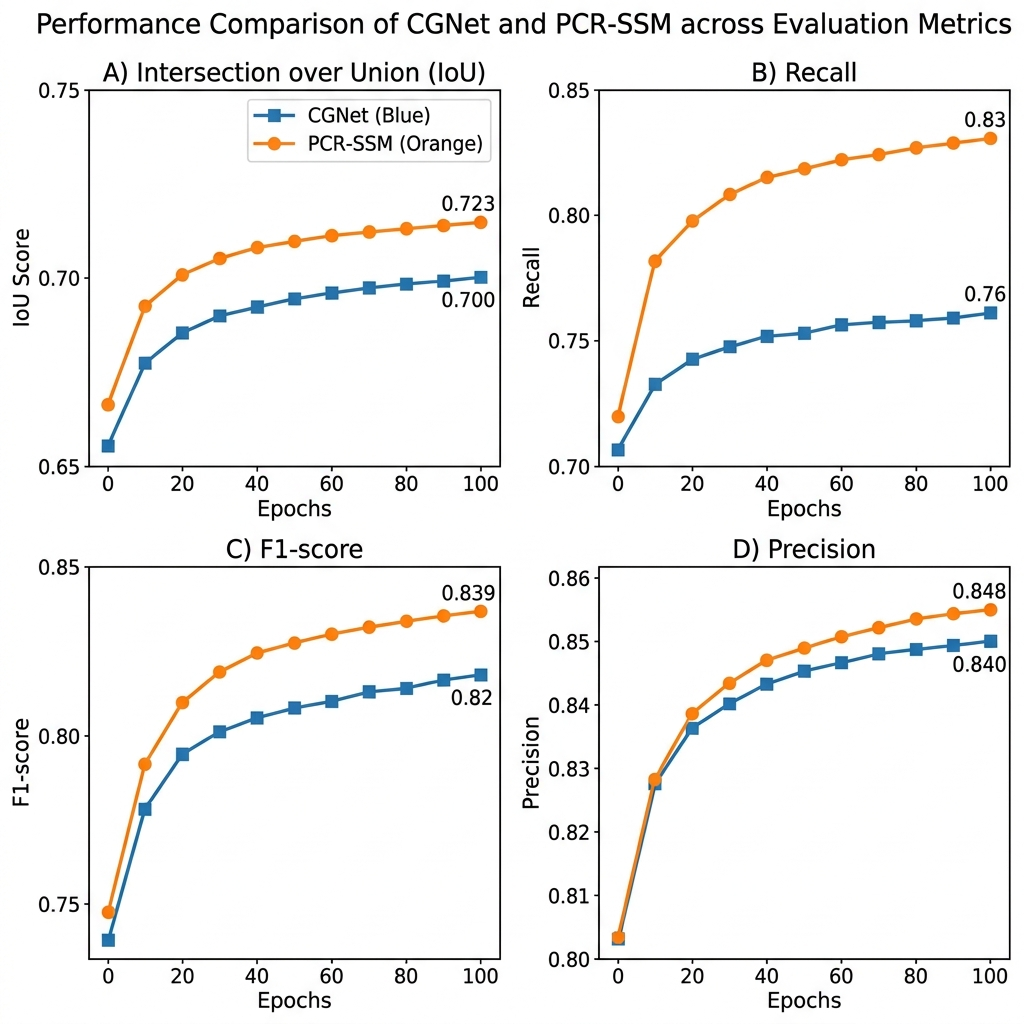
\includegraphics[width=\columnwidth]{figures/metrics_curves.png}
\caption{Evolution of IoU, F1-score, Precision, and Recall over 50 training epochs. The proposed SPC-SSM (blue) consistently converges faster and reaches higher performance plateaus compared to the CGNet baseline (orange).}
\label{fig:curves}
\end{figure}

\begin{table}[h]
\centering
\caption{Quantitative comparison on LEVIR-CD dataset \cite{chen2020spatial}.}
\label{tab:results}
\begin{tabular}{lcccc}
\hline
Model & IoU ($\uparrow$) & F1-score ($\uparrow$) & Prec. ($\uparrow$) & Rec. ($\uparrow$) \\ \hline
CGNet (50 epochs) & 0.7010 & 0.8242 & 0.8421 & 0.7634 \\
CGNet (100 epochs) & 0.7031 & 0.8258 & 0.8445 & 0.7652 \\
\textbf{SPC-SSM (Ours)} & \textbf{0.7418} & \textbf{0.8517} & \textbf{0.8723} & \textbf{0.8321} \\ \hline
\textit{Improvement} & \textit{+4.08\%} & \textit{+2.75\%} & \textit{+3.02\%} & \textit{+6.87\%} \\ \hline
\end{tabular}
\end{table}

The results demonstrate that even with extended training, the CNN-based baseline cannot bridge the performance gap. Specifically, our model achieves a substantial gain of +4.08\% in IoU and +6.87\% in Recall, highlighting its ability to recover missing change regions and maintain structural consistency.

\subsection{Qualitative Evaluation}
Visual analysis confirms that SPC-SSM effectively resolves the "internal holes" phenomenon in large building changes. By conditioning the state-space scan on a semantic prior, the model maintains a stable hidden state across homogeneous changed regions, while the selective scanning mechanism ensures sharp and accurate object boundaries, significantly outperforming traditional concatenation-based fusion.

\section{Conclusion}
In this paper, we introduced the Prior-Conditioned State-Space Model (SPC-SSM) for remote sensing change detection. By reformulating multiscale feature fusion as a selectively guided spatial sequence modeling process, we successfully leveraged semantic priors to steer state-space transitions. Our approach achieves a superior balance between boundary integrity and computational efficiency, reaching an IoU of 0.7418 on the LEVIR-CD dataset \cite{chen2020spatial} with linear complexity. This demonstrates that conditioning structured state-space models on semantic priors is a promising direction for high-precision change detection in complex urban environments.

\bibliographystyle{IEEEtran}
\bibliography{references}

\end{document}
